\documentclass[12pt]{report}
\usepackage{geometry} \geometry{a4paper, top=20mm, left=20mm, right=20mm, bottom=20mm, headsep=10mm, footskip=12mm} 
\usepackage[T1]{fontenc}
\usepackage[utf8]{inputenc}
\usepackage[english]{babel}
\usepackage{amsmath}
\usepackage{amsfonts}
\usepackage{amssymb}

\usepackage[bookmarks=true]{hyperref}
\usepackage{bookmark}
\usepackage{graphicx}
\usepackage{csvsimple}
\usepackage {multicol}


\usepackage{color}
\definecolor{keyword}{rgb}{0.5,0,0.35}		% keywords
\definecolor{comments}{rgb}{0.2,0.5,0.25}	% comments
\definecolor{identifier}{rgb}{0.2,0.2,0.2}	% identifiers

\usepackage{listings}
\lstset{numbers = left, 		% Position of line numbers
	basicstyle = \ttfamily ,% Font type
	keywordstyle = \color{keyword},	% style for keywords
	commentstyle = \color{comments}, % style for comments
	stringstyle = \color{identifier}, 
	numberstyle = \small, 	% Font style of numbers
	numbersep = 7pt, 		% Space between line number and code
	breaklines = true,		% Automatic line breaking
	tabsize = 4,				% number of spaces for TAB
	language = Java,		% Used language
	frame = single
}


\begin{document}
\title{Stocks Specification}			% put title in brackets
\author{Jan Veen}
\maketitle				% create headings
\cleardoublepage
\pdfbookmark{\contentsname}{Contents}
\tableofcontents

\chapter{Data Model}

\includegraphics[width=\linewidth]{diagrams/ER-diagram.png}

\section{Date formats}
What date format is used in which part of the system:

\begin{tabular}{l l}
Location & Format \\\hline
Client code & Localtime \\\hline
Client database & Localtime \\\hline
Network & UTC \\\hline
Server code & UTC \\\hline
Server database & UTC \\\hline
\end{tabular}

\chapter{Architecture}

\section{Used Software}

\section{Server}

\section{Client}

\subsection{Register New Data}

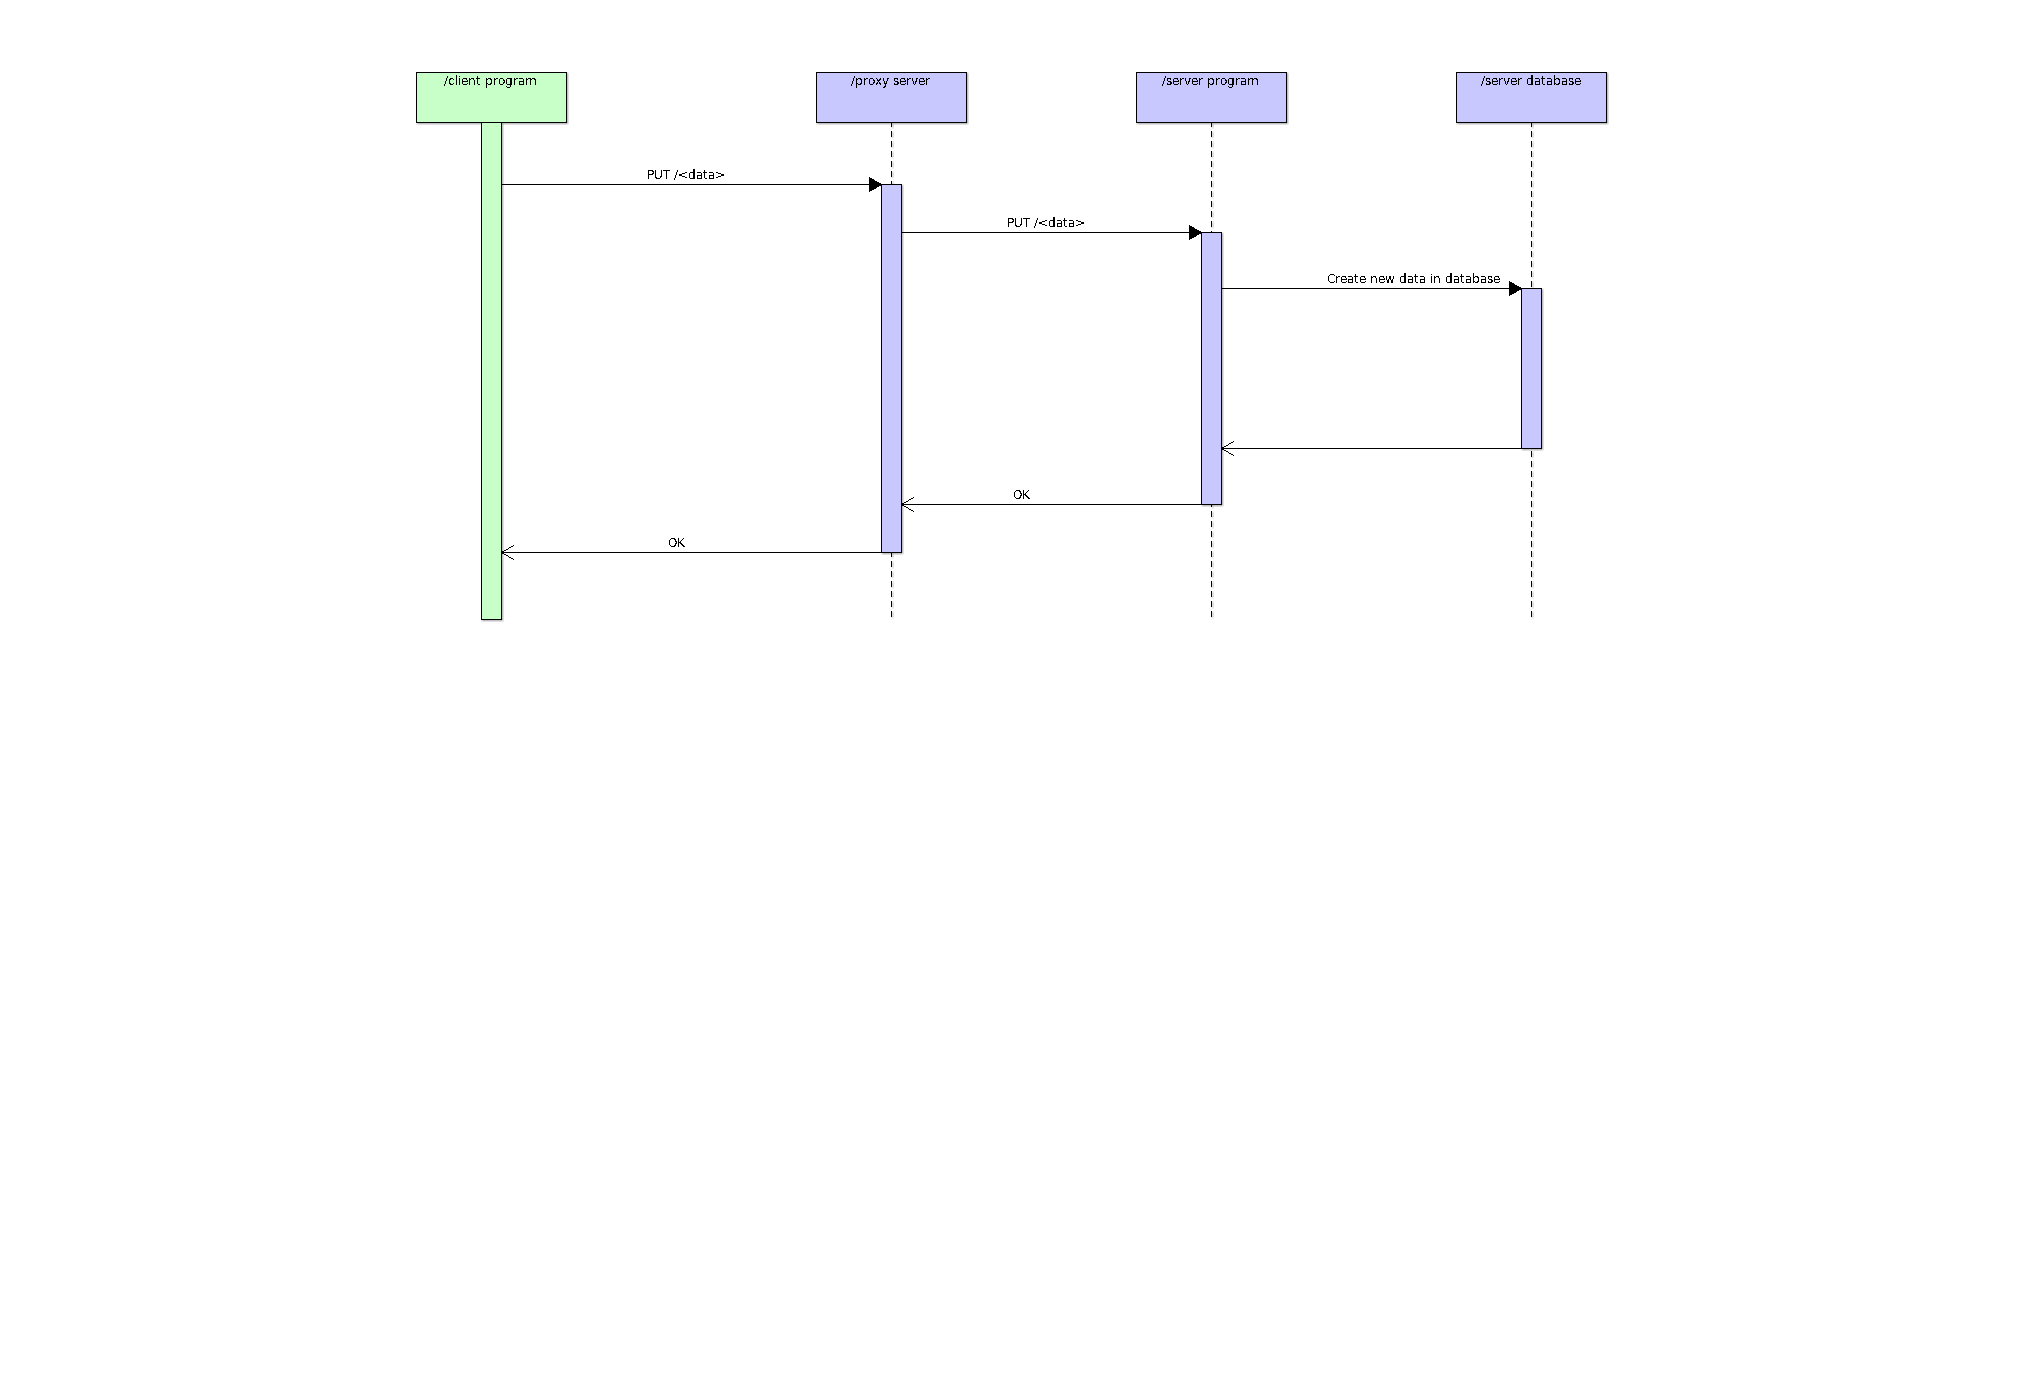
\includegraphics[width=\linewidth]{diagrams/put-data.png}

\subsection{Refresh client database}

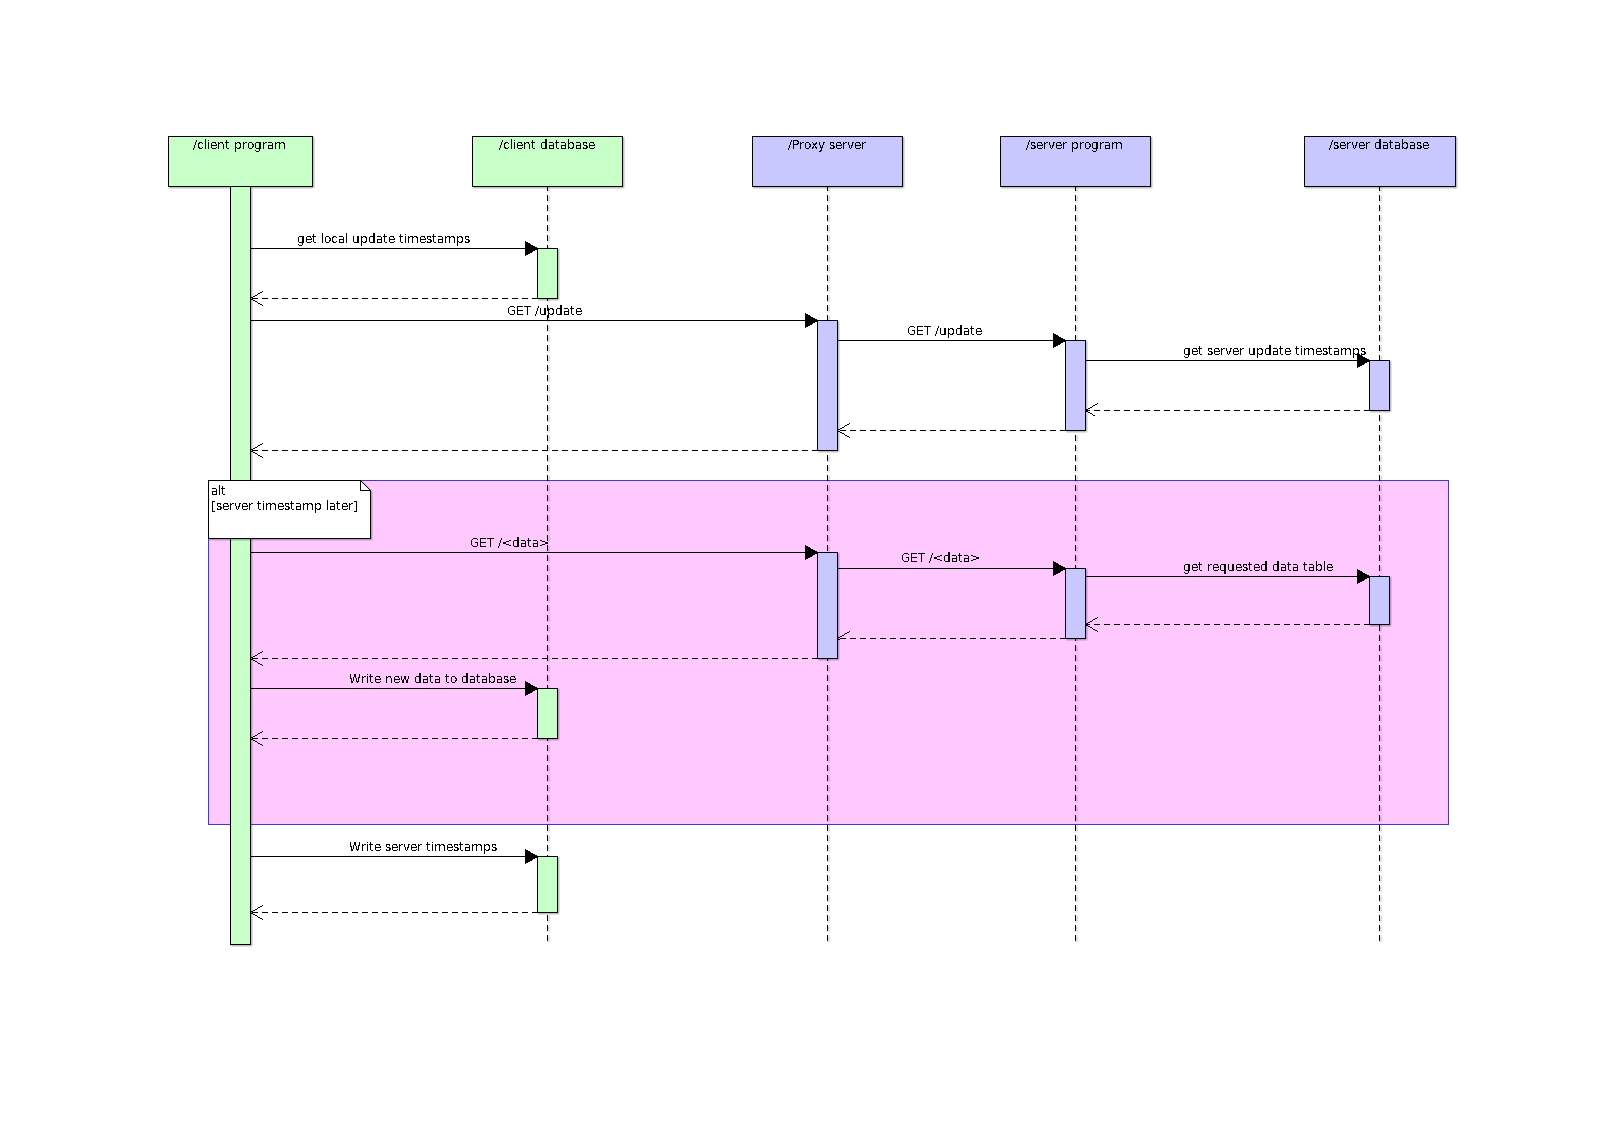
\includegraphics[width=\linewidth]{diagrams/Refreshment.png}

\subsection{New user registration}

New users are always added by giving a ticket from an existing user. The details are outlined in the diagram. 

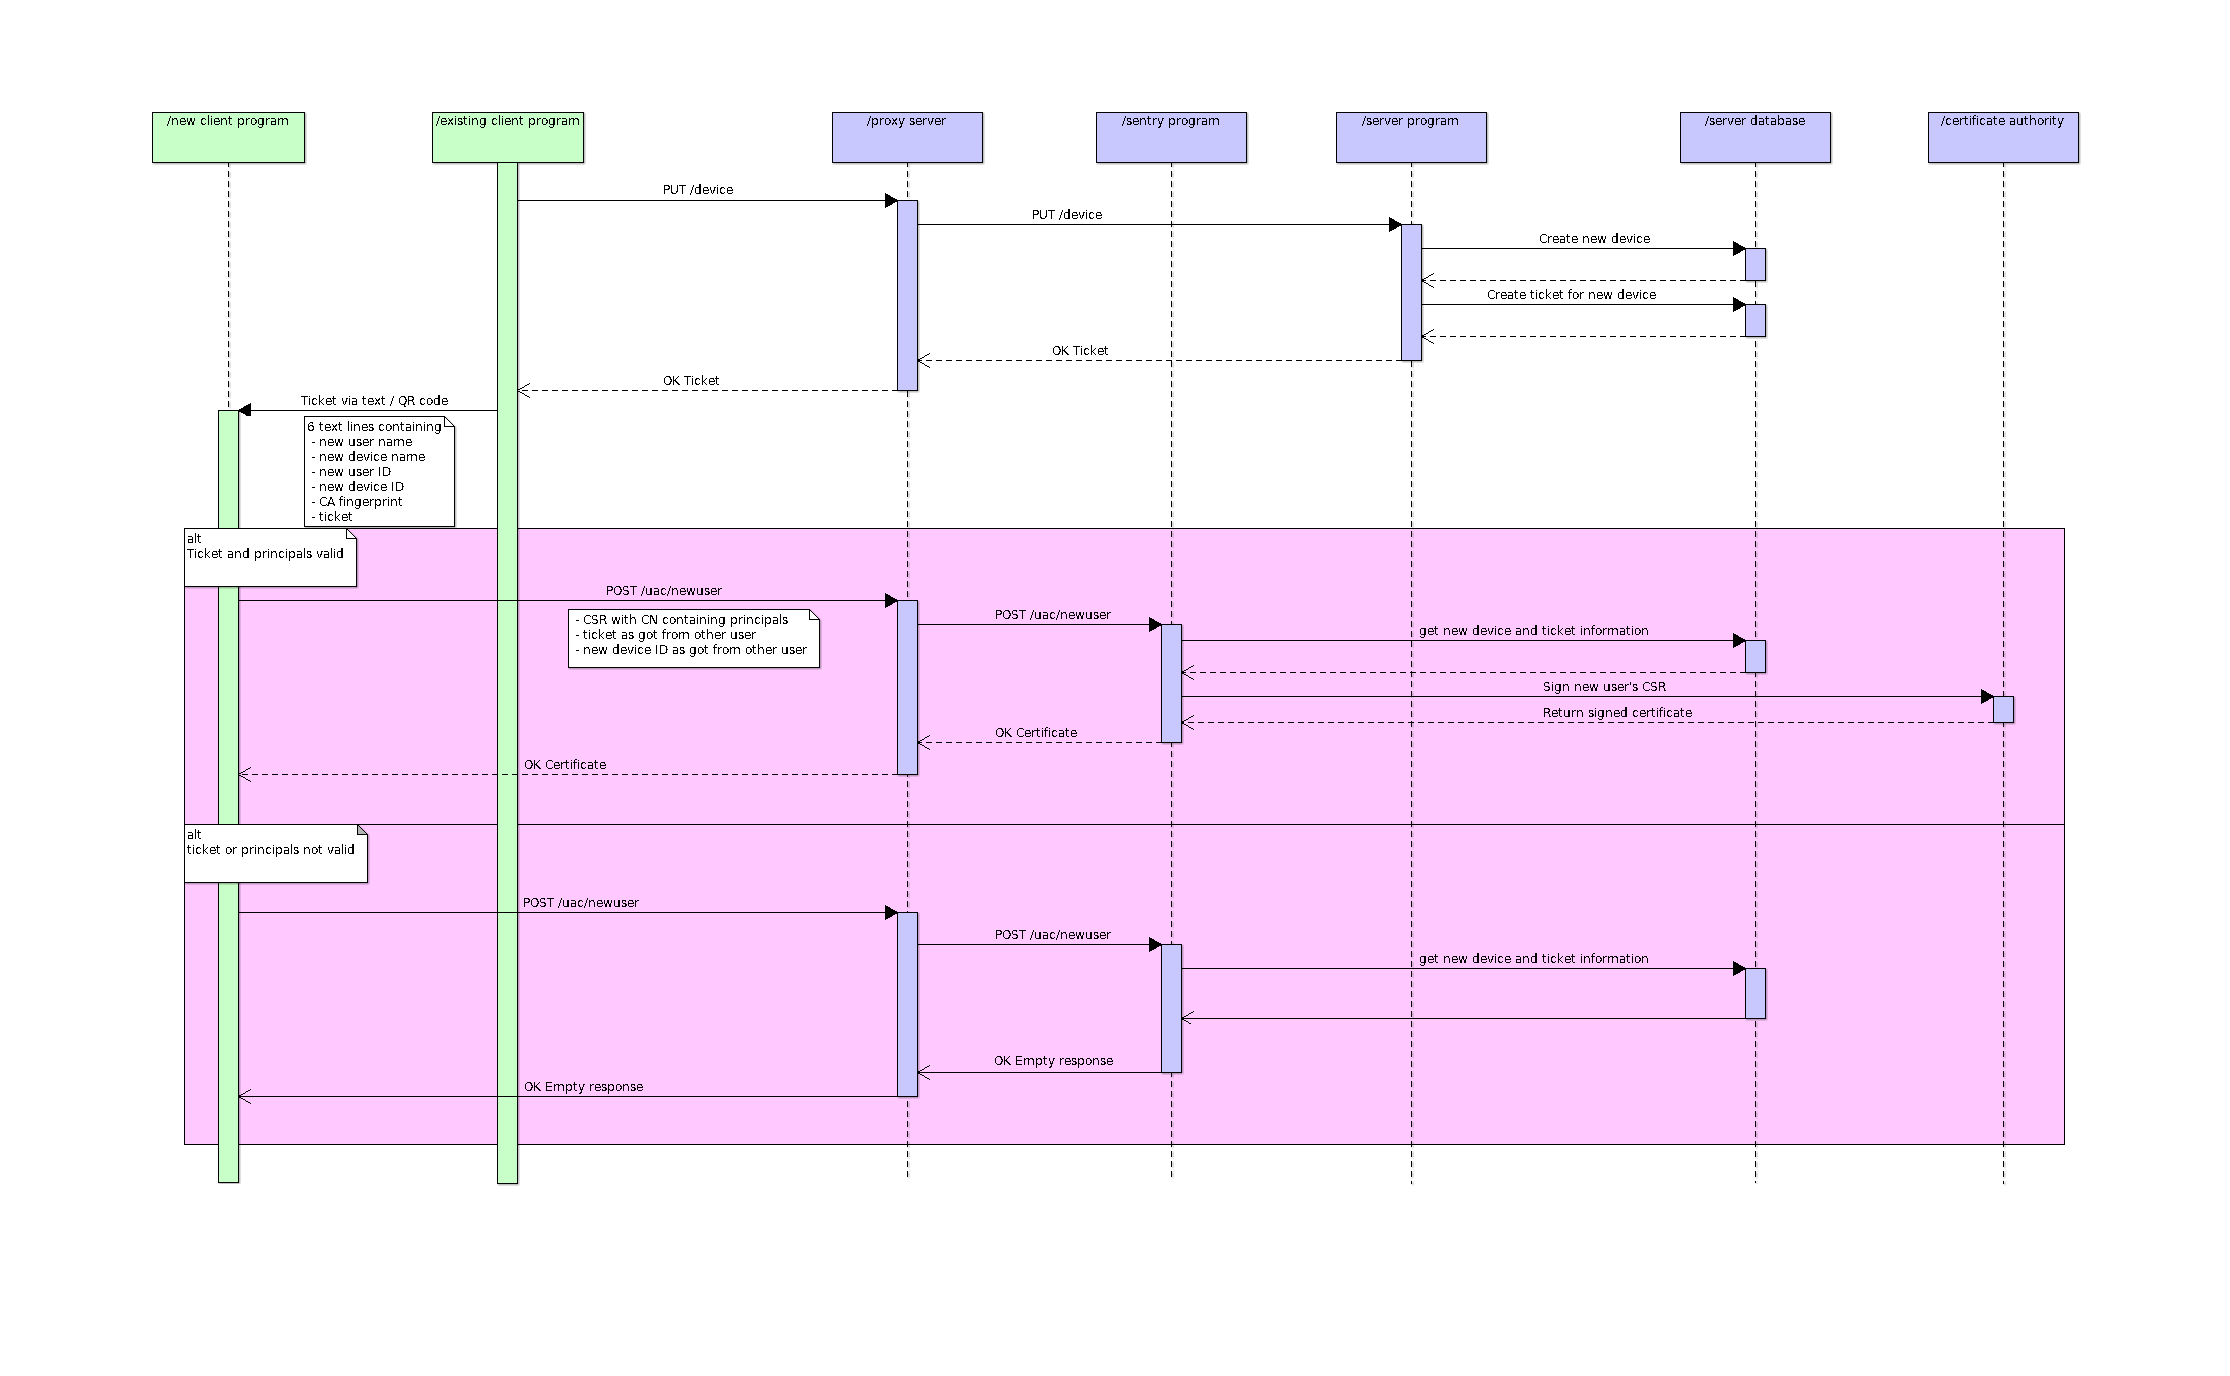
\includegraphics[width=\linewidth]{diagrams/new-user-registration.png}

\paragraph{Principal Names}
In the CSR the user stores the principals of his device. The values are formatted inside the Common Name attribute of the CSR. The pattern is \texttt{username\$user\_id\$ devicename\$device\_id}. So for the default test user this resolves to \texttt{John\$1\$Device\$1}. 
The principals are checked in the sentry part of the server before the certificate is signed. 

\paragraph{Client Verification}
Upon receiving a new device registration request, the sentry performs the following checks in order:
\begin{itemize}
\item Check if the ticket value presented by the client is found in the database
\item Check the device id associated with the ticket from the database with the device id from the CSR
\item Check if the remaining principals of the device match the CSR
\item Check if the ticket has expired
\end{itemize}
If all the checks succeed the sentry has the CSR signed by the CA and returns it to the client. 

\paragraph{QR Code Tickets}
For mobile clients it is more convenient to pass the ticket as QR code. To generate this QR code the content of the ticket has to be
entered text into the QR code. The order of the values is the same as in the diagram description. 

\subsection{Device removal}

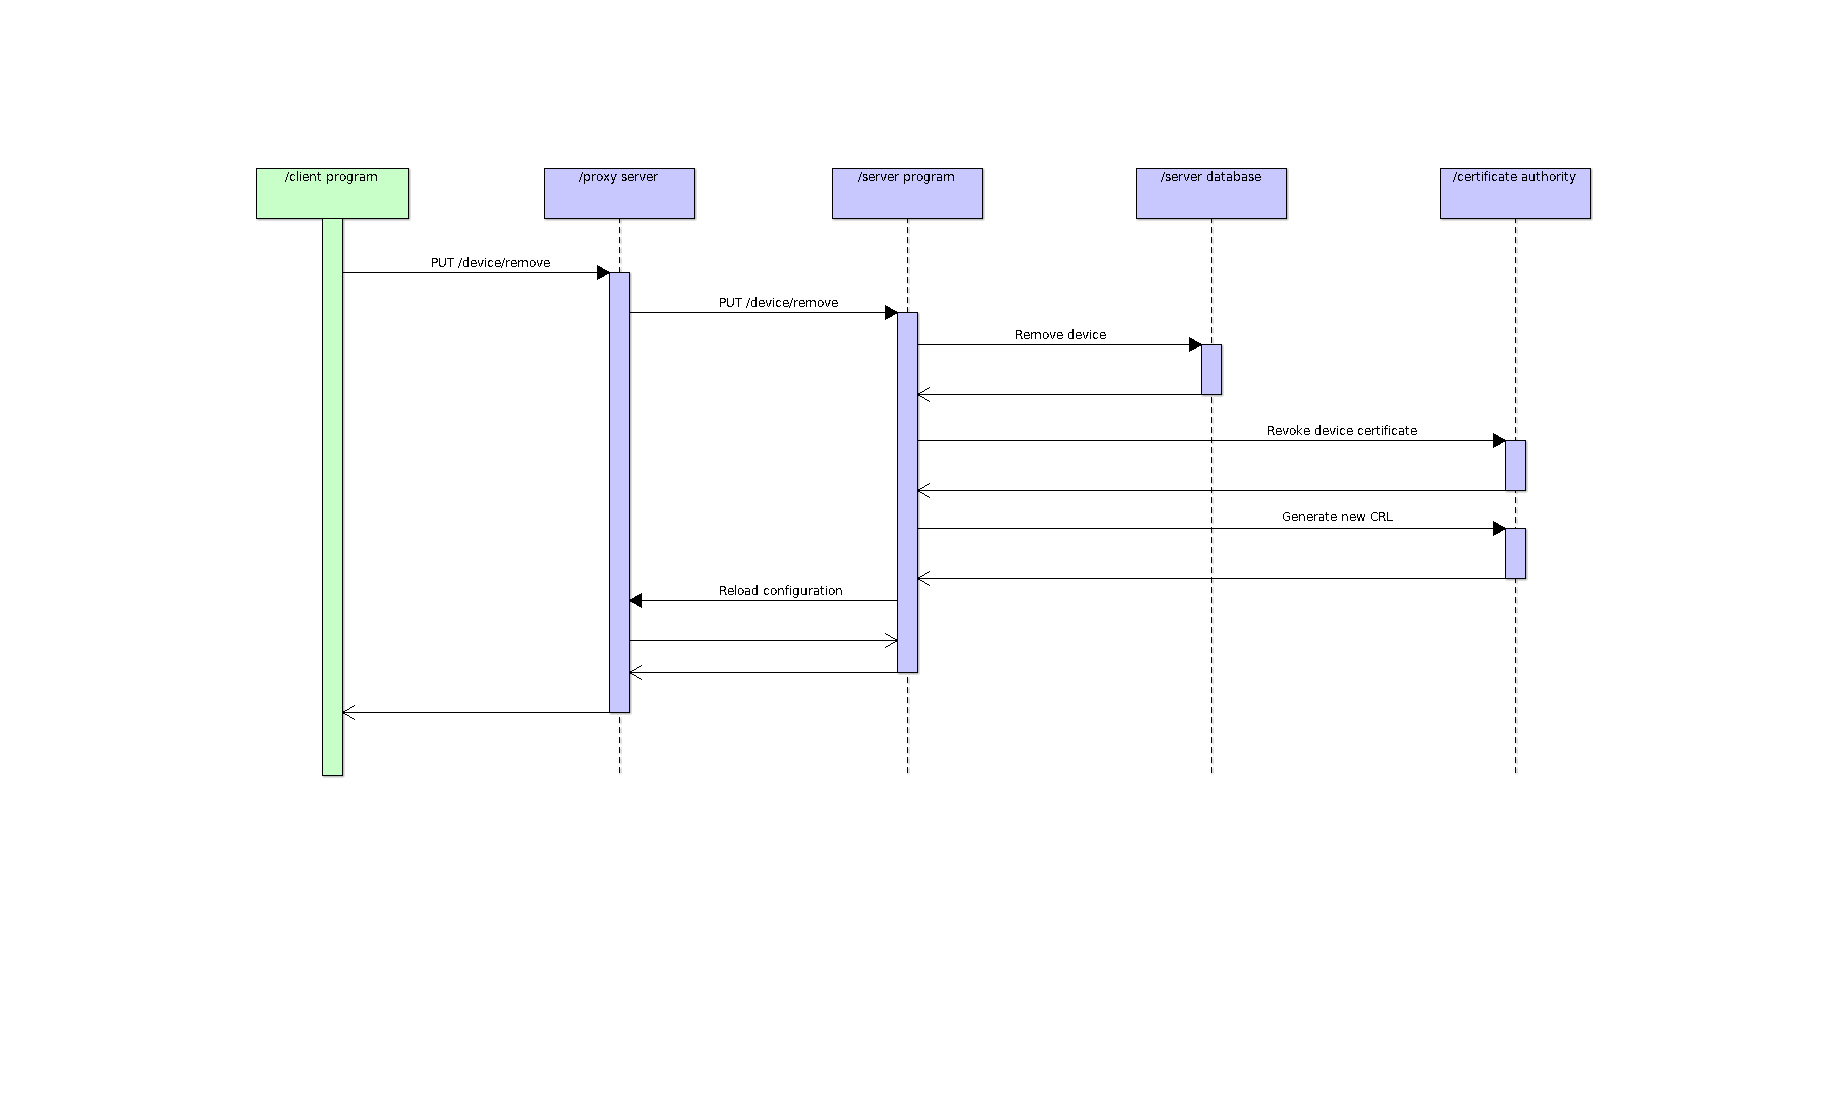
\includegraphics[width=\linewidth]{diagrams/remove-device.png}

\section{Security}







\end{document}
